% Copyright 2010 by Frank Wood

\documentclass[xcolor=dvipsnames]{beamer}
\usepackage{algorithm}
\usepackage{algorithmic}
\usepackage[]{natbib}

% Setup appearance:

\usetheme{Madrid}
%\usetheme{Copenhagen}
\usefonttheme[onlylarge]{structurebold}
\usecolortheme[RGB={0,63,135}]{structure} 
\setbeamerfont*{frametitle}{size=\normalsize,series=\bfseries}
%\setbeamertemplate{navigation symbols}{}

% Standard packages

\usepackage[english]{babel}
%\usepackage[latin1]{inputenc}
%\usepackage{times}
%\usepackage[T1]{fontenc}
%\usepackage{nnfootnote}
\usepackage{amsfonts}
\usepackage{amsmath}
\usepackage{xspace}

%\newcommand{\argmax}{\operatornamewithlimits{argmax}}
\def\newblock{\hskip .11em plus .33em minus .07em}
% Setup TikZ

%\usepackage{tikz}
%\usetikzlibrary{arrows}
%\tikzstyle{block}=[draw opacity=0.7,line width=1.4cm]



\defcitealias{Huggins-2012-AISTATS}{Huggins and W, 2011}
\defcitealias{Dewar:2011}{Dewar, Wiggins and W, 2011}


\newcommand{\eq}{\begin{equation*}}
\newcommand{\en}{\end{equation*}}
\newcommand{\eqa}{\begin{eqnarray*}}
\newcommand{\ena}{\end{eqnarray*}}
\newcommand{\eqn}{\begin{equation}}
\newcommand{\enn}{\end{equation}}
\newcommand{\eqan}{\begin{eqnarray}}
\newcommand{\enan}{\end{eqnarray}}
\newcommand{\GP}{$\Gamma$P}
\newcommand{\bsym}{\boldsymbol}

% Author, Title, etc.

\title[ISEDHMM] 
{
  Infinite Structured Explicit Duration \\
  Hidden Markov Models %\\ \small{~}\\ 
 % \tiny{How I Learned to Stop Worrying and Love the Infinite}
   % \tiny{A novel, general construction }
}

\author[Wood]
{
  Frank~Wood\\
  ~\\%\inst{1}\\
  \tiny{Joint work with Chris Wiggins, Mike Dewar, and \em{Jonathan Huggins}}
}

\institute[Columbia University]
{
  %\inst{1}%
  Columbia University
}

\date[November, 2011]
{November, 2011}

%\def\blfootnote{\xdef\@thefnmark{}\@footnotetext}


% The main document
% !TEX root = talk.tex

\newcommand{\comment}[1]{}
%\newcommand{\comment}[1]{{\marginpar{\tiny {#1} }}}
\def\todo#1{TODO(#1)}

\def\bigO{{\mathcal O}}
\def\balpha{\mbox{\boldmath $\alpha$}}
\def\bbeta{\mbox{\boldmath $\beta$}}
\def\beeta{\mbox{\boldmath $\eta$}}
\def\blambda{\mbox{\boldmath $\lambda$}}
\def\bmu{\mbox{\boldmath $\mu$}}
\def\bphi{\mbox{\boldmath $\phi$}}
\def\bpsi{\mbox{\boldmath $\psi$}}
\def\bsigma{\mbox{\boldmath $\sigma$}}
\def\btau{\mbox{\boldmath $\tau$}}
\def\btheta{\mbox{\boldmath $\theta$}}
\def\dbphi{\dot{\mbox{\boldmath $\phi$}}}
\def\dbtau{\dot{\mbox{\boldmath $\tau$}}}
\def\dbtheta{\dot{\mbox{\boldmath $\theta$}}}

%\newcommand{\nofootnotemark}{\let\@makefnmark\relax}
\newcommand{\bX}{\mathbf{X}}
\newcommand{\bY}{\mathbf{Y}}
\newcommand{\bW}{\mathbf{W}}
\newcommand{\bZ}{\mathbf{Z}}
\newcommand{\bH}{\mathbf{H}}
\newcommand{\bQ}{\mathbf{Q}}
\newcommand{\bA}{\mathbf{A}}
\newcommand{\bI}{\mathbf{I}}
\newcommand{\by}{\mathbf{y}}
\newcommand{\bz}{\mathbf{z}}
\newcommand{\bx}{\mathbf{x}}

\newcommand{\ith}{i^\mathrm{th}}
\def\A{{\bf A}}
\def\B{{\bf B}}
\def\C{{\bf C}}
\def\D{{\bf D}}
\def\F{{\bf F}}
\def\L{{\bf L}}
\def\M{{\bf M}}
\def\W{{\bf W}}
\def\I{{\bf I}}
\def\J{{\bf J}}
\def\R{{\bf R}}
\def\U{{\bf U}}
\def\V{{\bf V}}
\def\b{{\bf b}}
\def\c{{\bf c}}
\def\d{{\bf d}}
\def\r{{\bf r}}
\def\s{{\bf s}}
\def\t{{\bf t}}
\def\u{{\bf u}}
\def\v{{\bf v}}
\def\f{{\bf f}}
\def\x{{\bf x}}
\def\y{{\bf y}}
\def\w{{\bf w}}
\def\vo{{\bf o}}
\def\p{{\bf p}}
\def\O{{\bf 0}}
%\def\a{{\bf a}}


\def\vbpsi{\vec{\mbox{\boldmath $\psi$}}} 
\def\vpsi{\vec{\psi}} 
\def\vbphi{\vec{\mbox{\boldmath $\phi$}}} 
\def\vphi{\vec{\phi}} 
\def\vbtau{\vec{\mbox{\boldmath $\tau$}}} 
\def\vbtheta{\vec{\mbox{\boldmath $\theta$}}} 
\def\vD{\vec{D}}
\def\vf{\vec{\bf f}}
\def\vF{\vec{\bf F}}
\def\vI{\vec{\bf I}}
\def\vR{\vec{\bf R}}
\def\vv{\vec{v}}
\def\vV{\vec{\bf V}}

\def\pon{p_{\mathrm{on}}}
\def\poff{p_{\mathrm{off}}}

\def\tr{^{\text{T}}}

%%% Vector notation for sections 3 and 4
%%% Vector notation for sections 3 and 4
\def\mvec{\vec{m}}
\def\fvec{\vec{f}}
\def\appfvec{\vec{f}_k}
\def\avec{\vec{a}}
\def\bvec{\vec{b}}
\def\evec{\vec{e}}
\def\uvec{\vec{u}}
\def\xvec{\vec{x}}
\def\wvec{\vec{w}}
\def\gradvec{\vec{\nabla}}

\def\aM{\mbox{\bf a}_M}
\def\aS{\mbox{\bf a}_S}
\def\aO{\mbox{\bf a}_O}
\def\aL{\mbox{\bf a}_L}
\def\aP{\mbox{\bf a}_P}
\def\ai{\mbox{\bf a}_i}
\def\aj{\mbox{\bf a}_j}
\def\an{\mbox{\bf a}_n}
\def\a1{\mbox{\bf a}_1}
\def\a2{\mbox{\bf a}_2}
\def\a3{\mbox{\bf a}_3}
\def\a4{\mbox{\bf a}_4}

%\def\x{\mbox{\bf x\/}}
%\def\X{\mbox{\bf X}}
%\def\A{\mbox{\bf A}}
%\def\P{\mbox{\bf P}}
%\def\C{\mbox{\bf C}}
%\def\c{\mbox{\bf c}}
%\def\b{\mbox{\bf b}}
%\def\o{\mbox{\bf o}}
%\def\h{\mbox{\bf h}}
%\def\f{\mbox{\bf f}}
%\def\x{\mbox{\bf x}}
%\def\sx{\mbox{\scriptsize\bf x}}
%\def\z{\mbox{\bf z}}
%\def\l{\mbox{\bf l}}
%\def\m{\mbox{\bf m}}
%\def\bi{\mbox{\bf i}}
%\def\u{\mbox{\bf u}}
%\def\v{\mbox{\bf v}}
\def\a{\mbox{\bf a}}
%\def\p{\mbox{\bf p}}
%\def\r{\mbox{\bf r}}
%\def\d{\mbox{\bf d}}
%\def\Q{\mbox{\bf Q}}
%\def\s{\mbox{\bf s}}
%\def\st{\mbox{\scriptsize\bf t}}
%\def\ss{\mbox{\scriptsize\bf s}}
%\def\t{\mbox{\bf t}}
%\def\cR{{\cal R}}
%\def\calD{{\cal D}}
%\def\calS{{\cal S}}
%\def\g{\mbox{\bf g}}
%\def\e{\mbox{\bf e}}
%\def\flow{\{\mbox{\bf u}\}}
%\def\appearChange{iconic change}

\def\sigmae{\sigma}
\def\sigmam{\sigma}

\newcommand{\eg}{e.\thinspace{}g.,\@\xspace}
\newcommand{\egn}{e.\thinspace{}g.\@\xspace}
\newcommand{\cf}{cf.\@\xspace}
\newcommand{\ie}{i.\thinspace{}e.,\@\xspace}
\newcommand{\ien}{i.\thinspace{}e.\@\xspace}
\newcommand{\iid}{i.\thinspace{}i.\thinspace{}d.\@\xspace}


%\newcommand{\comment}[1]{}
\newcommand{\ponedec}{\mathcal{P}^\downarrow_1}
\newcommand{\pone}{\mathcal{P}_1}
\newcommand{\rank}[1]{\mathrm{RANK}\left[#1\right]}
\newcommand{\E}[1]{\mathrm{E}\left[#1\right]}
%\newcommand{\PY}{\mathcal{PY}}
%\newcommand{\DP}{\mathcal{DP}}
%\newcommand{\iid}{iid.}
\newcommand{\drawiid}{\stackrel{\text{iid}}{\sim}}
\newcommand{\vect}[1]{\mathbf{#1}}
\newcommand{\indicator}[1]{\text{I}\left[ #1 \right]}
\newcommand{\pdcoag}{PD(d_1,0)-\text{COAG}}
%\newcommand{\todo}{\textbf{*TODO*}}
\newcommand{\igram}{\text{$\infty$-gram}}
\newcommand{\Prob}{\text{P}}

\def\mm{sequence memoizer }
\def\MM{SM }

\def\pibf{{\boldsymbol{\pi}}}
\def\kapbf{\boldsymbol{\kappa}}
\def\taubf{\boldsymbol{\tau}}
\def\thebf{\boldsymbol{\theta}}
\def\rhobf{\boldsymbol{\rho}}
\def\phibf{\boldsymbol{\phi}}
\def\pbf{\mathbf{p}}
\def\qbf{\mathbf{q}}
\def\sbf{\mathbf{s}}
\def\tbf{\mathbf{t}}
\def\ybf{\mathbf{y}}
\def\ubf{\mathbf{u}}
\def\Ave{\mathbb{E}}

\def\wbf{\mathbf{w}}
\def\xbf{\mathbf{x}}
\def\rbf{\mathbf{r}}
\def\tbf{\mathbf{t}}
\def\kbf{\mathbf{k}}
\def\Xbf{\mathbf{X}}
\def\0bf{\mathbf{0}}
\def\Ibf{\mathbf{I}}
\def\phibf{\mathbf{\phi}}
\def\Phibf{\mathbf{\Phi}}
\def\disteq{{\stackrel{D}{=}}}
\def\EE{{\mathbb{E}}}
\def\GG{\mathcal{G}}
\def\G{G}
\def\U{U}

\def\phiv{\varphi}
\def\phivbf{\boldsymbol{\varphi}}

\def\Ocal{\mathcal{O}}
\DeclareMathOperator*{\Var}{Var}

\DeclareMathOperator*{\Bet}{Beta}
\DeclareMathOperator{\coag}{COAG}
\DeclareMathOperator{\frag}{FRAG}
\DeclareMathOperator*{\rnk}{RANK}
\DeclareMathOperator*{\gem}{GEM}
\DeclareMathOperator*{\pd}{PD}
\DeclareMathOperator*{\py}{PY}
\DeclareMathOperator*{\DP}{DP}
\DeclareMathOperator*{\PY}{PY}
\DeclareMathOperator*{\gd}{GDir}
\DeclareMathOperator*{\Dir}{Dir}
\DeclareMathOperator*{\CRP}{CRP}
\DeclareMathOperator*{\argmax}{argmax}



%%% Local Variables: 
%%% mode: latex
%%% TeX-master: "paper"
%%% End: 
% !TEX root = talk.tex
%
%\newcommand{\comment}[1]{}
%%\newcommand{\comment}[1]{{\marginpar{\tiny {#1} }}}
%
%\def\bigO{{\mathcal O}}
%\def\balpha{\mbox{\boldmath $\alpha$}}
%\def\bbeta{\mbox{\boldmath $\beta$}}
%\def\beeta{\mbox{\boldmath $\eta$}}
%\def\blambda{\mbox{\boldmath $\lambda$}}
%\def\bmu{\mbox{\boldmath $\mu$}}
%\def\bphi{\mbox{\boldmath $\phi$}}
%\def\bpsi{\mbox{\boldmath $\psi$}}
%\def\bsigma{\mbox{\boldmath $\sigma$}}
%\def\btau{\mbox{\boldmath $\tau$}}
%\def\btheta{\mbox{\boldmath $\theta$}}
%\def\dbphi{\dot{\mbox{\boldmath $\phi$}}}
%\def\dbtau{\dot{\mbox{\boldmath $\tau$}}}
%\def\dbtheta{\dot{\mbox{\boldmath $\theta$}}}
%
%%\newcommand{\nofootnotemark}{\let\@makefnmark\relax}
%\newcommand{\bX}{\mathbf{X}}
%\newcommand{\bY}{\mathbf{Y}}
%\newcommand{\bW}{\mathbf{W}}
%\newcommand{\bZ}{\mathbf{Z}}
%\newcommand{\bH}{\mathbf{H}}
%\newcommand{\bQ}{\mathbf{Q}}
%\newcommand{\bA}{\mathbf{A}}
%\newcommand{\bI}{\mathbf{I}}
%\newcommand{\by}{\mathbf{y}}
%\newcommand{\bz}{\mathbf{z}}
%\newcommand{\bx}{\mathbf{x}}
%
%\newcommand{\ith}{i^\mathrm{th}}
%\def\A{{\bf A}}
%\def\B{{\bf B}}
%\def\C{{\bf C}}
%\def\D{{\bf D}}
%\def\F{{\bf F}}
%\def\L{{\bf L}}
%\def\M{{\bf M}}
%\def\W{{\bf W}}
%\def\I{{\bf I}}
%\def\J{{\bf J}}
%\def\R{{\bf R}}
%\def\U{{\bf U}}
%\def\V{{\bf V}}
%\def\b{{\bf b}}
%\def\c{{\bf c}}
%\def\d{{\bf d}}
%\def\r{{\bf r}}
%\def\s{{\bf s}}
%\def\t{{\bf t}}
%\def\u{{\bf u}}
%\def\v{{\bf v}}
%\def\f{{\bf f}}
%\def\x{{\bf x}}
%\def\y{{\bf y}}
%\def\w{{\bf w}}
%\def\vo{{\bf o}}
%\def\p{{\bf p}}
%\def\O{{\bf 0}}
%%\def\a{{\bf a}}
%
%
%\def\vbpsi{\vec{\mbox{\boldmath $\psi$}}} 
%\def\vpsi{\vec{\psi}} 
%\def\vbphi{\vec{\mbox{\boldmath $\phi$}}} 
%\def\vphi{\vec{\phi}} 
%\def\vbtau{\vec{\mbox{\boldmath $\tau$}}} 
%\def\vbtheta{\vec{\mbox{\boldmath $\theta$}}} 
%\def\vD{\vec{D}}
%\def\vf{\vec{\bf f}}
%\def\vF{\vec{\bf F}}
%\def\vI{\vec{\bf I}}
%\def\vR{\vec{\bf R}}
%\def\vv{\vec{v}}
%\def\vV{\vec{\bf V}}
%
%\def\pon{p_{\mathrm{on}}}
%\def\poff{p_{\mathrm{off}}}
%
%\def\tr{^{\text{T}}}
%
%%%% Vector notation for sections 3 and 4
%%%% Vector notation for sections 3 and 4
%\def\mvec{\vec{m}}
%\def\fvec{\vec{f}}
%\def\appfvec{\vec{f}_k}
%\def\avec{\vec{a}}
%\def\bvec{\vec{b}}
%\def\evec{\vec{e}}
%\def\uvec{\vec{u}}
%\def\xvec{\vec{x}}
%\def\wvec{\vec{w}}
%\def\gradvec{\vec{\nabla}}
%
%\def\aM{\mbox{\bf a}_M}
%\def\aS{\mbox{\bf a}_S}
%\def\aO{\mbox{\bf a}_O}
%\def\aL{\mbox{\bf a}_L}
%\def\aP{\mbox{\bf a}_P}
%\def\ai{\mbox{\bf a}_i}
%\def\aj{\mbox{\bf a}_j}
%\def\an{\mbox{\bf a}_n}
%\def\a1{\mbox{\bf a}_1}
%\def\a2{\mbox{\bf a}_2}
%\def\a3{\mbox{\bf a}_3}
%\def\a4{\mbox{\bf a}_4}
%
%%\def\x{\mbox{\bf x\/}}
%%\def\X{\mbox{\bf X}}
%%\def\A{\mbox{\bf A}}
%%\def\P{\mbox{\bf P}}
%%\def\C{\mbox{\bf C}}
%%\def\c{\mbox{\bf c}}
%%\def\b{\mbox{\bf b}}
%%\def\o{\mbox{\bf o}}
%%\def\h{\mbox{\bf h}}
%%\def\f{\mbox{\bf f}}
%%\def\x{\mbox{\bf x}}
%%\def\sx{\mbox{\scriptsize\bf x}}
%%\def\z{\mbox{\bf z}}
%%\def\l{\mbox{\bf l}}
%%\def\m{\mbox{\bf m}}
%%\def\bi{\mbox{\bf i}}
%%\def\u{\mbox{\bf u}}
%%\def\v{\mbox{\bf v}}
%\def\a{\mbox{\bf a}}
%%\def\p{\mbox{\bf p}}
%%\def\r{\mbox{\bf r}}
%%\def\d{\mbox{\bf d}}
%%\def\Q{\mbox{\bf Q}}
%%\def\s{\mbox{\bf s}}
%%\def\st{\mbox{\scriptsize\bf t}}
%%\def\ss{\mbox{\scriptsize\bf s}}
%%\def\t{\mbox{\bf t}}
%%\def\cR{{\cal R}}
%%\def\calD{{\cal D}}
%%\def\calS{{\cal S}}
%%\def\g{\mbox{\bf g}}
%%\def\e{\mbox{\bf e}}
%%\def\flow{\{\mbox{\bf u}\}}
%%\def\appearChange{iconic change}
%
%\def\sigmae{\sigma}
%\def\sigmam{\sigma}
%
%\newcommand{\eg}{e.\thinspace{}g.,\@\xspace}
%\newcommand{\egn}{e.\thinspace{}g.\@\xspace}
%\newcommand{\cf}{cf.\@\xspace}
%\newcommand{\ie}{i.\thinspace{}e.,\@\xspace}
%\newcommand{\ien}{i.\thinspace{}e.\@\xspace}
%\newcommand{\iid}{i.\thinspace{}i.\thinspace{}d.\@\xspace}
%
%
%%\newcommand{\comment}[1]{}
%\newcommand{\ponedec}{\mathcal{P}^\downarrow_1}
%\newcommand{\pone}{\mathcal{P}_1}
%\newcommand{\rank}[1]{\mathrm{RANK}\left[#1\right]}
%%\newcommand{\E}[1]{\mathrm{E}\left[#1\right]}
%%\newcommand{\PY}{\mathcal{PY}}
%%\newcommand{\DP}{\mathcal{DP}}
%%\newcommand{\iid}{iid.}
%\newcommand{\drawiid}{\stackrel{\text{iid}}{\sim}}
%\newcommand{\vect}[1]{\mathbf{#1}}
%\newcommand{\indicator}[1]{\text{I}\left[ #1 \right]}
%\newcommand{\pdcoag}{PD(d_1,0)-\text{COAG}}
%%\newcommand{\todo}{\textbf{*TODO*}}
%\newcommand{\igram}{\text{$\infty$-gram}}
%\newcommand{\Prob}{\text{P}}
%
%\def\mm{sequence memoizer }
%\def\MM{SM }
%
%\def\pibf{{\boldsymbol{\pi}}}
%\def\kapbf{\boldsymbol{\kappa}}
%\def\taubf{\boldsymbol{\tau}}
%\def\thebf{\boldsymbol{\theta}}
%\def\rhobf{\boldsymbol{\rho}}
%\def\phibf{\boldsymbol{\phi}}
%\def\pbf{\mathbf{p}}
%\def\qbf{\mathbf{q}}
%\def\sbf{\mathbf{s}}
%\def\tbf{\mathbf{t}}
%\def\ybf{\mathbf{y}}
%\def\ubf{\mathbf{u}}
%\def\Ave{\mathbb{E}}
%
%\def\wbf{\mathbf{w}}
%\def\xbf{\mathbf{x}}
%\def\rbf{\mathbf{r}}
%\def\tbf{\mathbf{t}}
%\def\kbf{\mathbf{k}}
%\def\Xbf{\mathbf{X}}
%\def\0bf{\mathbf{0}}
%\def\Ibf{\mathbf{I}}
%\def\phibf{\mathbf{\phi}}
%\def\Phibf{\mathbf{\Phi}}
%\def\disteq{{\stackrel{D}{=}}}
%\def\GG{\mathcal{G}}
%\def\G{G}
%\def\U{U}
%
%\def\phiv{\varphi}
%\def\phivbf{\boldsymbol{\varphi}}
%
%\def\Ocal{\mathcal{O}}
%\DeclareMathOperator*{\Var}{Var}
%
%\DeclareMathOperator*{\Bet}{Beta}
%\DeclareMathOperator{\coag}{COAG}
%\DeclareMathOperator{\frag}{FRAG}
%\DeclareMathOperator*{\rnk}{RANK}
%\DeclareMathOperator*{\gem}{GEM}
%\DeclareMathOperator*{\pd}{PD}
%\DeclareMathOperator*{\py}{PY}
%\DeclareMathOperator*{\DP}{DP}
%\DeclareMathOperator*{\PY}{PY}
%\DeclareMathOperator*{\gd}{GDir}
%\DeclareMathOperator*{\Dir}{Dir}
%\DeclareMathOperator*{\CRP}{CRP}
%\DeclareMathOperator*{\argmax}{argmax}
%
\def\GG{\mathcal{G}}
\def\data{\mathbf{x}}
%\def\EE{\mathbb{E}}
\def\disc{d}
%\newcommand{\delete}[1]{} %\textcolor{red}{#1}
%\newcommand{\rewrite}[1]{#1}%{\textcolor{blue}{#1}} %
%\newcommand{\lambdabf}{\boldsymbol{\lambda}}
%\newcommand{\vbf}{\mathbf{v}}
%\newcommand{\Psmooth}{\Prob_\text{smooth}}
%%\newcommand{\parent}{\pi}
%\newcommand{\suffix}{\sigma}
%\newcommand{\UHPYP}{SM}
%\newcommand{\PLUMP}{PLUMP}
%\newcommand{\Oh}{\mathcal{O}}
%\newcommand{\tree}{\mathcal{T}}
\newcommand{\cct}{\hat{\mathcal{T}}}
\newcommand{\cctx}{\cct(\data)}
\newcommand{\Gu}{G_{\ubf}}
%\newcommand{\GuSet}{\{G_{\ubf}\}_{\ubf \in \Sigma^*}}
%\newcommand{\E}{\mathrm{E}}
%\newcommand{\UpdatePath}{\text{\textsc{UpdatePath}}}
%\newcommand{\Path}{\ensuremath{(\ubf_0,\ldots,\ubf_P)}}
%\newcommand{\PathProbability}{\text{\textsc{PathProbability}}}
%\newcommand{\TT}{\mathcal{T}}
%\newcommand{\ral}[1]{\stackrel{\mathtt{#1}}{\rightarrow}}
\def\parent{{\sigma(\mathbf{u})}}
%
%%\def\newblock{\hskip .11em plus .33em minus .07em}
%
%
%% \newcommand{\cusk}{c_{\ubf s k}}
%% \newcommand{\cus}{c_{\ubf s \cdot}}
%% \newcommand{\cu}{c_{\ubf \cdot \cdot}}
%% \newcommand{\tus}{t_{\ubf s}}
%% \newcommand{\tu}{t_{\ubf \cdot}}
%\newcommand{\cusk}{c_{\ubf s k}}
%\newcommand{\cus}{c_{\ubf s}}
%\newcommand{\cu}{c_{\ubf \cdot}}
%\newcommand{\tus}{t_{\ubf s}}
%\newcommand{\tu}{t_{\ubf \cdot}}
%\newcommand{\cset}{\{\cusk\}_{s\in \Sigma,k \in \{1,\ldots,t_{\ubf s}\}}}
%\newcommand{\tset}{\{\tus\}_{s\in \Sigma}}
%\newcommand{\bydef}{\equiv}
%\newcommand{\state}{\mathcal{S}_{\xbf}}
%\newcommand{\statei}{\mathcal{S}_{\xbf_{1:i}}}
%%\newcommand{\emptystring}{\varepsilon}
%\newcommand{\gcount}{\hat{c}}
%\newcommand{\escape}{\mathtt{esc}}
%\def\prob{G}
%
%
%\newcommand{\todo}[1]{\begin{center}\textbf{TODO: } #1 \end{center}}
%\newcommand{\figref}[1]{\figurename~\ref{#1}}
%\newcommand{\predictive}{\Prob(x_i|\xbf_{1:i-1})}
%\newcommand{\ywcomment}[1]{\textbf{#1}}
%\newcommand{\jgcomment}[1]{ { \textcolor{red}{#1} } }
%
%\newcommand{\secref}[1]{Section \ref{#1}}
%
\def\context{\mathbf{u}}

%%% Local Variables: 
%%% mode: latex
%%% TeX-master: "paper"
%%% End: 


\usebackgroundtemplate{
\includegraphics[width=\paperwidth]{../columbia_background.png}}

\begin{document}

%\nofootnotemark
\begin{frame}
  \titlepage
\end{frame}

%\begin{frame}{Outline}
%  \tableofcontents
% \end{frame}
%\section{Background}
%\frame[t] {
%\frametitle{Probabilistic Modeling}
%Data
%\[ \bsym y = (y_{1}, \dots, y_{T})\]
%Latent Variables (extensive in the data)
%\[\bsym z = (z_{1}, \dots, z_{T})\]
%Parameters (fixed size with respect to data)
%\[\Theta\]
%}
%
%\frame[t] {
%\frametitle{Probabilistic Modeling}
%Data
%\[ \bsym y = (y_{1}, \dots, y_{T})\]
%Latent Variables (extensive in the data)
%\[\bsym z = (z_{1}, \dots, z_{T})\]
%Parameters (fixed size with respect to data)
%\[\Theta\]
%}


\frame[t] {
\frametitle{Hidden Markov Models}
Hidden Markov models (HMMs) \citep{Rabiner:1989} are an important tool for data exploration and engineering applications.
\newline

Applications include
\begin{itemize}
\item Speech recognition \citep{Jelinek97,Juang85}
\item Natural language processing \citep{Manning1999}
\item Hand-writing recognition \citep{Nag1986}
\item DNA and other biological sequence modeling applications \citep{Krogh1994}
\item Gesture recognition \citep{tanguay1995hidden,wilson1999parametric}
\item Financial data modeling \citep{ryden1998stylized}
\item $\ldots$ and many more.\newline

\end{itemize}

%Assumptions: discrete time, latent Markov process.

}

%\begin{frame}[t]{Example Application: Modeling the Morse Code Cepstrum}
%	\begin{figure}[t]
%		\begin{center}
%			\includegraphics[height = 6cm, transparent]{figs/morse-spectrogram-ED-iHMM-and-iHMM-output}
%		\end{center}
%	\end{figure}
%\end{frame}

\frame[t] {
\frametitle{Graphical Model: Hidden Markov Model}
\begin{figure}[t]
		\begin{center}
			\includegraphics[width = \textwidth, transparent]{figs/HMM-graphical-model}
		\end{center}
	\end{figure}
%An objective: compute the predictive distribution for the next observation:
%\eqan
%\lefteqn{P(y_T | y_1,\ldots, y_{T-1}, \{{\bsym\pi}_m\},\{\theta_m\})} \nonumber \\
%&=& \sum_{z_T}\sum_{z_{T-1}}\cdots\sum_{z_0} p(y_T | z_T) p(z_T | z_{T-1}) \ldots p(y_{1})p(z_{1} | z_{0}) p(z_0) \nonumber
%\enan
}

\frame[t] {
\frametitle{Notation: Hidden Markov Model}

\eqan
%\theta_{m} &\sim& H_{y} \nonumber \\
\!\!\!\!\! z_{t} | z_{t-1}=m &\sim&
	\mathsf{Discrete}(\bsym\pi_{m})
	\nonumber \\
y_{t} | z_{t}=m &\sim& F_{\theta}(\theta_{m})\nonumber
\enan

\[\mathbf{A} = \left[ \begin{array}{ccccc}
	\vdots & & \vdots & & \vdots \\
	\bsym\pi_{1} &\cdots& \bsym\pi_{m} &\cdots& \bsym\pi_{K} \\
	\vdots & & \vdots & & \vdots \\
	\end{array} \right]
\]
}

%\frame[t] {
%\frametitle{Notation: Hidden Markov Model, Choices for $F_{\theta}$}
%
%\begin{description}
%\item[ $F_{\theta} = \mathsf{Multinomial(\Theta)}$] 
%discrete observations (i.e.~DNA, words, etc.)
% \[\theta_{m} \; \mbox{is a probability vector}\] 
% \item[$F_{\theta} = \mathsf{Normal(\Theta)}$] 
% continuous observations (i.e.~positions, etc.). \[\theta_{m}  = \{\mu_m, \Sigma_m\}\]
%\end{description}
%
%
%
%%We define the observation sequence $\mathcal{Y} = \{y_1, y_2, \ldots, y_T\}$; the latent state sequence $\mathcal{X} = \{x_0, x_1, x_2, \ldots, x_T\}$; and the remaining time in each segment $\mathcal{D} = \{ d_1, d_2, \ldots, d_T\}$, where $x_t \in \{ 1, 2, \ldots, K\}$ with $K$ the maximum number of states, $d_t \in \{1, 2, \ldots \}$, and $y_t \in \mathbb{R}^n$.     We assume that the Markov chain on the latent states is homogenous, i.e., that $p(x_t = i | x_{t-1}=j, A) = a_{i,j} \forall t$ where $A$ is a $K\times K$ matrix with element $a_{i,j}$ at row $i$ and column $j.$  
%
%}

%\frame[t] {
%\frametitle{ HMM: Dynamic mixture model}
% \begin{figure}[t]
%		\begin{center}
%			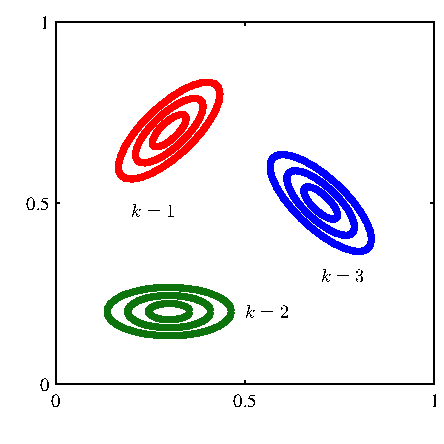
\includegraphics[width = .5\textwidth, transparent]{figs/Figure13_8a}
%			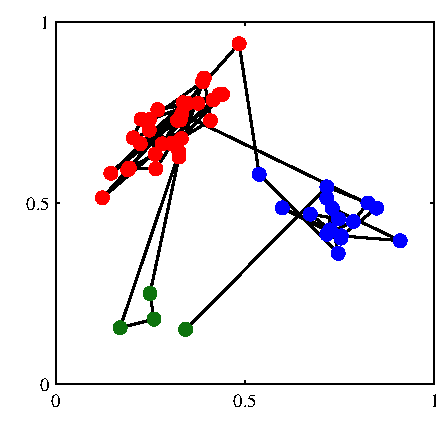
\includegraphics[width = .5\textwidth, transparent]{figs/Figure13_8b}
%		\end{center}
%	\end{figure}
%	Visualization from PRML. \citep{Bishop06}
%
%}

%\frame[t] {
%\frametitle{ HMM: Trellis}
% \begin{figure}[t]
%		\begin{center}
%			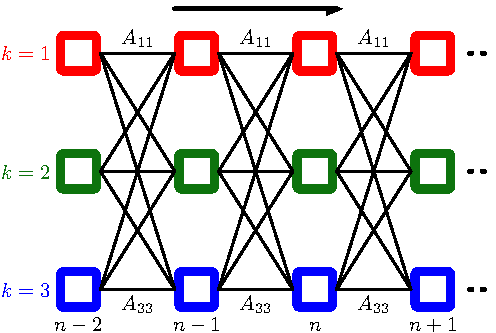
\includegraphics[width = .7\textwidth, transparent]{figs/Figure13_7}
%		\end{center}
%	\end{figure}
%	Visualization from PRML. \citep{Bishop06}
%
%}


\frame[t] {
\frametitle{HMM: Typical Usage Scenario (Character Recognition)}
\begin{itemize}
\item Training data: multiple ``observed''  $y_t = \{v_t,h_t\}$ sequences of stylus positions for each kind of character %(stroke boundaries unobserved but important ``structurally'' --- correspond to latent states)
\item Task: train $|\Sigma|$ different models, one for each character %(Maximum likelihood training via EM: {\em Baum-Welch} \citep{baum1972equality}, {\em forward-backward} \citep{Rabiner:1989}, belief propagation \citep{Bishop06})
\item Latent states: sequences of strokes 
\item Usage: classify new stylus position sequences using trained models  $\mathcal{M}_\sigma = \{A_\sigma, \Theta_\sigma\}$% and Bayes factors
\[ P(  \mathcal{M}_\sigma | y_1,\ldots,y_T) \propto P(y_1,\ldots,y_T | \mathcal{M}_\sigma) P( \mathcal{M}_\sigma) \]
 %which requires marginalizing out $z$'s 
%\[ P(y_1,\ldots,y_T | \mathcal{M}_\sigma) = \sum_Z P(y_1,\ldots,y_T, z_0, \ldots, z_T | A_\sigma, \Theta_\sigma)\]
\end{itemize}

}

\frame[t] {
\frametitle{Shortcomings of Original HMM Specification}
\begin{itemize}
\item Latent state dwell times are not usually geometrically distributed
\eqan
\lefteqn{P(z_{t} = m, \ldots, z_{t+L} = m | A)} \nonumber \\
 &=& \prod_{\ell = 1}^L P(z_{t+\ell+1} = m| z_{t+\ell} = m, A) \nonumber \\
 &=& \mathsf{Geometric}(L; \bsym\pi_m(m)) \nonumber
 \enan
\item Prior knowledge often suggests structural constraints on allowable transitions
\item The state cardinality of the latent Markov chain $K$ is usually unknown
\end{itemize}

}

\section{Related Work}

\frame[t] {
\frametitle{Explicit Duration HMM / H. Semi-Markov Model}
\citep{Mitchell95,Murphy02,Yu03,Yu:2010}
\begin{itemize}
\item Latent state sequence $\bsym z = (\{s_{1},r_1\},\dots, \{s_{T},r_T\})$
\item Latent state id sequence $\bsym s = (s_{1},\dots, s_{T})$
\item Latent ``remaining duration'' sequence $\bsym r = (r_{1},\dots, r_{T})$
%\item Observation sequence $\bsym y = (y_{1}, \dots, y_{T})$
\item State-specific duration distribution $F_{r}(\lambda_{m})$
%\item State transition matrix with columns $\bsym \pi_{m} = (\pi_{m1},\pi_{m2},\dots, \pi_{mM})$
%\item State-specific observation distribution $y_{t} \sim F_{\theta}(\theta_{m})$
\item Other distributions the same
\end{itemize}

An EDHMM transitions between states in a different way than does a typical HMM. Unless $r_{t} = 0$  the current remaining duration is decremented and the state does not change.  If $r_{t} = 0$ then the EDHMM transitions to a state $m \ne s_{t}$ according to the distribution defined by $\bsym \pi_{s_{t}}$ 

%A finite explicit duration HMM (EDHMM) consists of a hidden state sequence $\bsym s = (s_{1},\dots, s_{T})$, the corresponding observation sequence $\bsym y = (y_{1}, \dots, y_{T})$, and a latent ``remaining duration'' sequence $\bsym r = (r_{1},\dots, r_{T})$.  It also has a state transition matrix  $\bsym \pi$, where the row vector $\bsym \pi_{m} = (\pi_{m1},\pi_{m2},\dots, \pi_{mM})$ corresponds to the transition probabilities out of state $m$, and $\bsym \pi_{0}$ is the initial state vector. An EDHMM transitions between states in a different way than does a typical HMM. Unless $r_{t} = 0$  the current remaining duration is decremented and the state does not change.  If $r_{t} = 0$ then the EDHMM transitions to a state $m \ne s_{t}$ according to the distribution defined by $\bsym \pi_{s_{t}}$. The duration the HMM will remain in the new state $m$ is drawn from the  state-specific duration distribution $F_{r}(\lambda_{m})$ governed by parameter $\lambda_{m}$. At each timestep the observation $y_{t} \sim F_{\theta}(\theta_{m})$ is drawn from a state-specific emission distribution parameterized by $\theta_{m}$.   The emission distribution parameters are given a shared prior $\theta_m \sim H_{\theta}$. The IEDHMM is an EDHMM with a countable number of states, i.e.~$M\rightarrow\infty$.


}

\frame[t] {
\frametitle{EDHMM notation}

Latent state $z_t = \{s_t, r_t\}$ is tuple consisting of state identity and time left in state.

\eqan
%\theta_{m} &\sim& H_{\theta} \nonumber \\
%\lambda_{m} &\sim& H_{r}\nonumber \\
\!\!\!\!\! s_{t} | s_{t-1}, r_{t-1} &\sim& 
	\begin{cases} 
	\mathbb I(s_{t} = s_{t-1}), & \! r_{t-1} > 0 \\
	\mathsf{Discrete}(\bsym\pi_{s_{t-1}}), & r_{t-1} = 0
	\end{cases}\nonumber \\
\!\!\!\!\! r_{t } | s_{t}, r_{t-1} &\sim& 
	\begin{cases} 
	\mathbb I(r_{t} = r_{t-1} - 1),& r_{t-1} > 0 \\
	F_{r}(\lambda_{s_{t}}),& r_{t-1} = 0
	\end{cases} \nonumber\\
y_{t} | s_{t} &\sim& F_{\theta}(\theta_{s_{t}})\nonumber
\enan


}

\frame[t] {
\frametitle{EDHMM: Graphical Model}
\begin{figure}[t]
		\begin{center}
			\includegraphics[width = \textwidth, transparent]{figs/EDHMM-graphical-model}
		\end{center}
	\end{figure}
}





\frame[t] {
\frametitle{Structured HMMs: i.e.~left-to-right HMM \citep{Rabiner:1989}}

\begin{block}{Example: Chicken pox}
\begin{description}
\item[Observations] vital signs
\item[Latent states] pre-infection, infected, post-infection\footnote{disregarding shingles} 
\item[State transition structure]  can't go from infected to pre-infection
\end{description}
\end{block}
Structured transitions imply zeros in the transition matrix $A$, i.e.

\[p(s_t = m | s_{t-1} = \ell) = 0 \; \forall \; m < \ell\]


}


%\frame[t] {
%\frametitle{Structured HMM: Trellis: One step at a time, left-to-right HMM }
%
% \begin{figure}[t]
%		\begin{center}
%			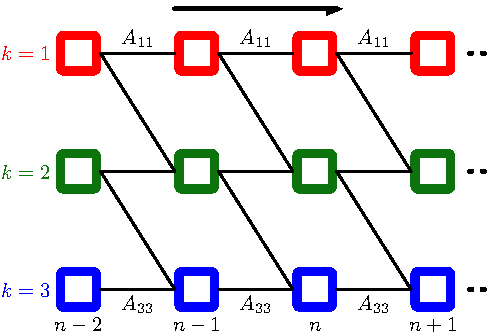
\includegraphics[width = .7\textwidth, transparent]{figs/Figure13_10}
%		\end{center}
%	\end{figure}
%	Figure from PRML. \citep{Bishop06}
%
%}

\frame[t] {
\frametitle{Bayesian HMM}

\begin{itemize}
\item We will put a {\em prior} on parameters so that we can effect a solution that conforms to our  ideas about what the solution should look like 

\begin{itemize}
\item Structured prior examples
\begin{itemize}
\item $A_{i,j}=0$ (hard constraints)
\item $A_{i,j}\approx \sum_j A_{i,j}$ (rich get richer)
\end{itemize}
\end{itemize}


\item  {\em Regularization} means that we can specify a model with more parameters than could possibly be needed
\begin{itemize}
\item infinite complexity  (i.e.~$K \rightarrow \infty$) avoids many model selection problems
\item  ``extra'' states can be thought of as auxiliary or nuisance variables 
\end{itemize}
%\item  Posterior inference treats parameters $A$ and $\Theta$ as latent variables

\end{itemize}


}

%\frame[t] {
%\frametitle{Bayesian HMM}
% Posterior inference treats parameters as latent variables and marginalizes them out too. \newline
%
%%Consider the earlier sequence classification task, now
%
%%\[P(\{y_1,\ldots,y_T\}^{\mbox{new}} |  \]
%%
%%\[ P(  \mathcal{M}_\sigma | y_1,\ldots,y_T) \propto P(y_1,\ldots,y_T | \mathcal{M}_\sigma) P( \mathcal{M}_\sigma) \]
%% which requires marginalizing out $z$'s {\em and} $A$ and $\Theta$
%%\eqan
%%\lefteqn{P(y_1,\ldots,y_T | \mathcal{H})}\nonumber \\
%%&=& \int \int \sum_Z P(y_1,\ldots,y_T, z_0, \ldots, z_T,  A_\sigma, \Theta_\sigma| \mathcal{H}) dP(A_\sigma) dP(\Theta_\sigma)
%%\enan
%%where $\mathcal{H}$ is a set of hyperparameters.
%
%
%
%}

\frame[t] {
\frametitle{Bayesian HMM}
\begin{figure}[t]
		\begin{center}
			\includegraphics[width = \textwidth, transparent]{figs/Bayesian-HMM-graphical-model}
		\end{center}
	\end{figure}
%
\alert<1>{\eqan
\bsym\pi_{m} &\sim& H_{z} \nonumber \\
\theta_{m} &\sim& H_{y} \nonumber 
\enan}%
\eqan
\!\!\!\!\! z_{t} | z_{t-1}=m &\sim&
	\mathsf{Discrete}(\bsym\pi_{m})
	\nonumber \\
y_{t} | z_{t}=m &\sim& F_{\theta}(\theta_{m})\nonumber
\enan
}


\frame[t] {
\frametitle{Infinite HMMs (IHMM) \citep{Beal:2002,Teh:2006b}}
 
 
 
 \begin{figure}[t]
		\begin{center}
			\includegraphics[width = \textwidth, transparent]{figs/iHMM-graphical-model}
		\end{center}
	\end{figure}
	  \[K \rightarrow \infty\]

}

\frame[t] {
\frametitle{Other HMM variants}
\begin{itemize}
\item Sticky Infinite HMMs \citep{Fox:2010tg}
\begin{itemize}
\item Extra parameter per state used to bias towards self-transition
\end{itemize}
\item Hierarchical HMMs \citep{Murphy01a} 
\begin{itemize}
\item State is hierarchical (i.e.~sequence of letters composed of stroke sequences)
\end{itemize}
\item  Factorial HMMs \citep{Ghahramani96a}
%\begin{itemize}
%\item State is binary encoding 
%\end{itemize}
\item  Infinite explicit duration HMM \citep{Johnson:2010}
\begin{itemize}
\item No generative model. Latent history sampling used to assert the existence of an implicitly defined IEDHMM that can be sampled from by rejecting HDP-HMM samples that violate transition constraints.
\end{itemize}
\end{itemize}

}

\section{ISEDHMMs}




\frame[t] {
\frametitle{Infinite Structured Explicit Duration HMM (ISEDHMM) }

Generative framework for HMMs with
\begin{itemize}
\item Explicitly parameterized duration distributions
\item Structured transition priors
\item Countable state cardinality
\end{itemize}
Fundamental Problems
\begin{itemize}
\item How to generate {\em structured, dependent, infinite-dimensional} transition distributions.
%\begin{itemize}
%\item Example: explicit duration HMM's require no self-transitions \[\bsym\pi_i(i)=A_{i,i}=0\]
%\item HDP-HMM construction good for dependence, doesn't work for structure
%\end{itemize}
%The HDP-HMM construction of the iHMM  \citep{Teh:2006b, VanGael:2008} would seem to be a good way to construct an IEDHMM. 
%In sich a construction each row of $\bsym\pi$ (of which there a countably infinite number) would be a draw from a Dirichlet process (DP) with base measure $D_{0} = \sum_{k=1}^{\infty} w_{k}\delta_{\theta_{k}}$, where $D_{0}$ is itself a draw from a Dirichlet process with base measure $H_{\theta}$.
%Therefore, the $m$-th draw $D_{m} \sim \textnormal{DP}(c_{0}D_{0})$ can be written as $D_{m} = \sum_{k} \pi_{mk}\delta_{\theta_{k}}$. 
%Unfortunately the IEDHMM cannot be constructed in this manner because the HPD-HMM cannot enforce the kind of dependence required by the no self-transition condition $m \ne s_{t}$.  This is because the HDP prior on the transition distributions requires that any time a state is transitioned to from any other state it becomes more likely to be transitioned to by all other states.  Unfortunately developing a a model in which the state transition distributions exhibit dependence on a covariate or auxiliary variable requires the abandoning the conditional independence requirement of the HDP.
\item How to do inference in HMMs with countable state cardinality and countable duration distribution support.
\end{itemize}
\;\;\;\;\;\;\citepalias{Huggins-2012-AISTATS}
}

\begin{frame}[t]{ ISEDHMM: Graphical Model}
	\begin{figure}[t]
		\begin{center}
			\includegraphics[height = 5cm, transparent]{figs/ED-iHMM-graphical-model}
		\end{center}
	\end{figure}
	
	{\em Structured, dependent, infinite-dimensional} transition distributions?
\end{frame}

\frame[t] {
\frametitle{ISEDHMM: Recipe}
\begin{itemize}
\item Poisson process \citep{Kingman:1993} 
\item Gamma process \citep{Kingman:1993} 
\item SN\GP s \citep{Rao:2009}
\item {\em Structured, dependent, infinite-dimensional} transition distributions \citepalias{Huggins-2012-AISTATS}
\end{itemize}

}

\frame[t] {
\frametitle{ISEDHMM: Recipe}

\begin{itemize}
\item Gamma process  \citep{Kingman:1993} as Poisson process over $\Theta \otimes V \otimes [0,\infty)$ with rate / mean measure
\eqn \mu(\tilde\Theta, \tilde V,  \tilde S) = \alpha(\tilde\Theta, \tilde V) \int_{\tilde S}\gamma^{-1}e^{-\gamma} \nonumber \enn
\item A draw from a Gamma process with \[\alpha(\tilde\Theta,  \tilde V) = c_{0}H_{\theta}(\tilde\Theta)H_{v}( \tilde V).\] \citep{Kingman:1993} has the form
\eqn G  = \sum_{m=1}^{\infty} \gamma_{m} \delta_{(\theta_{m}, v_{m})} \nonumber \enn
where $(\theta_{m}, v_{m}) \sim H_{\theta}\times H_{v}$. \newline
\end{itemize}

}
\frame[t] {
\frametitle{ISEDHMM: Recipe}
\begin{itemize}
\item Non-disjoint ``restricted projections'' of Gamma processes are {\em dependent} Gamma processes (SN\GP s) \citep{Rao:2009}
\begin{figure}[t]
		\begin{center}
			\includegraphics[width=.75\textwidth, transparent]{figs/isedhmm_geom_base_gp}
		\end{center}
	\end{figure}
	
	\end{itemize}

\eqn G_0 = \sum_{m\neq0} \ldots, \;\;\;\cdots\;\;\;,G_4  = \sum_{m\neq4} \gamma_{m} \delta_{\theta_{m}},\;\;\;\cdots\;\;\;  \nonumber \enn

}
	
	
\frame[t] {
\frametitle{ISEDHMM: Recipe}

	\begin{itemize}

\item Normalized dependent \GP~draws are dependent Dirichlet process draws.\footnote{a draw from a Dirichlet process \citep{Ferguson1973} is an infinite sum of weighted atoms \citep{Sethuraman1994} where the weights sum to one.}  In the ISEDHMM, DP draws are the dependent, structured, infinite-dimensional transition distributions

\eqan D_4  &=& \frac{G_4}{G_4(\Theta)} \\
 &=& \frac{\sum_{m\neq4} \gamma_{m} \delta_{\theta_{m}}}{\sum_{\theta \in \Theta}\sum_{m'\neq4} \gamma_{m'} \delta_{\theta_{m'}}} \\
 &=& \frac{\sum_{m\neq4} \gamma_{m} \delta_{\theta_{m}}}{\sum_{m'\neq4} \gamma_{m'}}\\
 &=& \sum_{m\neq4} \frac{\gamma_{m}}{\sum_{m'\neq4} \gamma_{m'}} \delta_{\theta_{m}} \nonumber \enan
	\end{itemize}

}

\frame[t] {
\frametitle{ISEDHMM: Recipe}
	\begin{figure}[t]
		\begin{center}
			\includegraphics[height = 6cm, transparent]{figs/ED-iHMM-hierarchical-model}
		\end{center}
	\end{figure}
	
	\begin{itemize}

\item Structured, dependent, infinite dimensional transition distributions $\bsym\pi_m$ can be formed from draws from DDPs \citepalias{Huggins-2012-AISTATS}
%\item Auxiliary variables
%\item Beam Sampling
\end{itemize}
}

%\begin{frame}[t]{IEDHMM: Geometric base distribution over states example}
%	\end{frame}

%\frame[t] {
%\frametitle{Structured Transitions Via Dependent Dirichlet Processes}
%\begin{itemize}
%\item<1-3> One way to define a set of dependent DPs is to construct a base gamma process over an augmented space by taking the union of disjoint independent gamma processes, then define a series of restricted projections of that base process, which are themselves gamma processes. 
%
%\item<2-3> The normalization of these dependent gamma processes form a set of dependent DPs.  
%
%\item<3-3> We will use this procedure to construct a number of dependent DPs (one for each HMM state) which preclude certain transitions.  The precluded transitions, a form of dependence,  arise from particulars.
%\end{itemize}
%
%}


\frame[t] {
\frametitle{ISEDHMM Inference: Beam Sampling}
We employ the forward-filtering, backward slice-sampling approach for the IHMM of \citep{VanGael:2008} and EDHMM of \citepalias{Dewar:2011}, %This so-called beam sampling approach is an auxiliary variable slice-sampling approach. 
in which the state and duration variables $\bsym s$ and $\bsym r$ are sampled conditioned on auxiliary slice variables $\bsym u$. \newline % via a forward-chainin 

Net result: efficient, always finite forward backward procedure for sampling latent states.

}



\frame[t] {
\frametitle{Auxiliary Variables for Sampling}
\begin{columns}[t]
\begin{column}{.5\textwidth}

Objective: get samples of $x$.  \newline 

\uncover<2->{Sometimes it is easier to introduce an auxiliary variable $u$ and to Gibbs sample the joint $P(x,u)$ (i.e.~sample from $P(x|u; \lambda)$ then $P(u|x, \lambda)$, etc.) then discard the $u$ values than it is to directly sample from $p(x|\lambda)$. \newline}%

\uncover<3->{Useful when: $p(x|\lambda)$ does not have a known parametric form but adding $u$ results in a parametric form {\em and} when $x$ has countable support and sampling it requires enumerating all values. }

	\end{column}
	\begin{column}{.25\textwidth}
\uncover<1->{\begin{figure}[t]
		\begin{center}
			\includegraphics[height = 3cm, transparent]{figs/poisson_slice_sampling_example_before_aux}
		\end{center}
	\end{figure}
	}
	\end{column}
		\begin{column}{.25\textwidth}

	\uncover<2->{\begin{figure}[t]
		\begin{center}
			\includegraphics[height = 5cm, transparent]{figs/poisson_slice_sampling_example}
		\end{center}
	\end{figure}
	}
	\end{column}
	\end{columns}


}




\frame[t] {
\frametitle{Slice Sampling: A {\em very} useful auxiliary variable sampling trick}
Unreasonable Pedagogical Example: 
\begin{itemize}
\item $x|\lambda \sim \mathsf{Poisson}(\lambda)$ (countable support)
\item  {\em enumeration} strategy for sampling $x$ (impossible)
\item auxiliary variable $u$ with $P(u|x,\lambda) = \frac{\mathbb{I}(0 \leq u \leq P(x|\lambda))}{P(x|\lambda)}$
\end{itemize}
Note:
Marginal distribution of $x$ is 
\eqan
P(x|\lambda) &=& \sum_u P(x,u|\lambda) \nonumber\\
&=& \sum_u P(x|\lambda)P(u|x,\lambda) \nonumber\\
&=& \sum_u P(x|\lambda) \frac{\mathbb{I}(0 \leq u \leq P(x|\lambda))}{P(x|\lambda)}\nonumber\\
&=& \sum_u \mathbb{I}(0 \leq u \leq P(x|\lambda)) = P(x|\lambda) \nonumber
\enan

}

\frame[t] {
\frametitle{Slice Sampling: A {\em very} useful auxiliary variable sampling trick}
This suggests a Gibbs sampling scheme: alternately sampling from
\begin{itemize}
\item $P(x|u,\lambda) \propto \mathbb{I}(u \leq P(x|\lambda))$ 
\begin{itemize}
\item {\em finite} support, uniform above slice, enumeration {\em possible}
\end{itemize}
\item  $P(u|x,\lambda) = \frac{\mathbb{I}(0 \leq u \leq P(x|\lambda))}{P(x|\lambda)}$ 
\begin{itemize}
\item uniform between 0 and $y=P(x|\lambda)$
\end{itemize}
\end{itemize}
then discarding the $u$ values to arrive at $x$ samples marginally distributed according to $P(x|\lambda)$.
}

\frame[t] {
\frametitle{ISEDHMM Inference: Beam Sampling}
Forward-backward slice sampling only has to consider a finite number of successor states at each timestep.  With auxiliary variables

\eqn p(u_{t} | z_{t}, z_{t-1}) = \frac{\mathbb I(u_{t} < p(z_{t} | z_{t-1}))}{ p(z_{t} | z_{t-1})} \nonumber \enn

and

\eqan
 p(z_{t} | z_{t-1}) &=&
 p((s_t , r_t ) | (s_{t-1}, r_{t-1}))  \nonumber \\
	&=&\begin{cases} 
	r_{t-1} > 0, & \mathbb{I}(s_t=s_{t-1})\mathbb{I}(r_t = r_{t-1}-1) \\
	r_{t-1} = 0, & \pi_{s_{t-1}s_{t}}F_r(r_t;\lambda_{s_t}).
	\end{cases} \nonumber 
\enan

one can run standard forward-backward conditioned on $u$'s.
}

\frame[t] {
\frametitle{Results}
To illustrate IEDHMM learning on synthetic data, five hundred datapoints were generated using a 4 state EDHMM with Poisson duration distributions \[\bsym \lambda = (10, 20, 3, 7)\] and Gaussian emission distributions with means \[\bsym \mu = (-6, -2, 2, 6)\] all unit variance. 
}

\begin{frame}[t]{IEDHMM: Synthetic Data Results}
	\begin{figure}[t]
		\begin{center}
			\includegraphics[height = 7cm, transparent]{figs/combined-overlay-state-distribution-figure}
		\end{center}
	\end{figure}
\end{frame}

\begin{frame}[t]{IEDHMM: Synthetic Data, State Duration Parameter Posterior }
	\begin{figure}[t]
		\begin{center}
			\includegraphics[height = 6cm, transparent]{figs/4-states-4-apart-1-variance-duration-posteriors-big-font}
		\end{center}
	\end{figure}
\end{frame}

\begin{frame}[t]{IEDHMM: Synthetic Data, State Mean Posterior}
	\begin{figure}[t]
		\begin{center}
			\includegraphics[height = 6cm, transparent]{figs/4-states-4-apart-1-variance-mean-posteriors-big-font}
		\end{center}
	\end{figure}
\end{frame}

\begin{frame}[t]{IEDHMM: Nanoscale Transistor Spontaneous Voltage Fluctuation}
	\begin{figure}[t]
		\begin{center}
			\includegraphics[height = 6cm, transparent]{figs/RTS-ED-iHMM-overlay}
		\end{center}
	\end{figure}
\end{frame}



\begin{frame}[t]{IEDHMM vs. IHMM:  Modeling the Morse Code Cepstrum}
	\begin{figure}[t]
		\begin{center}
			\includegraphics[height = 6cm, transparent]{figs/morse-spectrogram-ED-iHMM-and-iHMM-output}
		\end{center}
	\end{figure}
\end{frame}



\begin{frame}[t]{Wrap-Up}
\begin{itemize}
\item Novel Gamma process construction for dependent, structured, infinite dimensional HMM transition distributions.
\item Other transition distribution structures (left-to-right) can be implemented simply by changing ``restricted projection regions.''
\item ISEDHMM framework generalizes the HMM, Bayesian HMM, infinite HMM, left-to-right HMM, explicit duration HMM, and more.
\end{itemize}

\end{frame}

\begin{frame}[t]{Future Work}
\begin{itemize}
\item Generalize to spatial prior on HMM states (``location'')
\begin{itemize}
\item Simultaneous location and mapping
\item Process diagram modeling for systems biology
\end{itemize}
\item Applications; seeking ``users''
\end{itemize}

\end{frame}

\begin{frame}[t]{Questions?}

Thank you!

\end{frame}



%\frame[t] {
%\frametitle{HMM as PNFA}
%}
%
%\frame[t] {
%\frametitle{Computational Models of Worlds}
%}
%
%\frame[t] {
%\frametitle{Sequence Memoizer}
%}
%
%\frame[t] {
%\frametitle{Probabilistic Deterministic Infinite Automata}
%}
%
%
%
%\begin{frame}[t]{Sequence Memoizer graphical model ``oacac" \cite{Wood2009}}
%	\begin{figure}[t]
%		\begin{center}
%			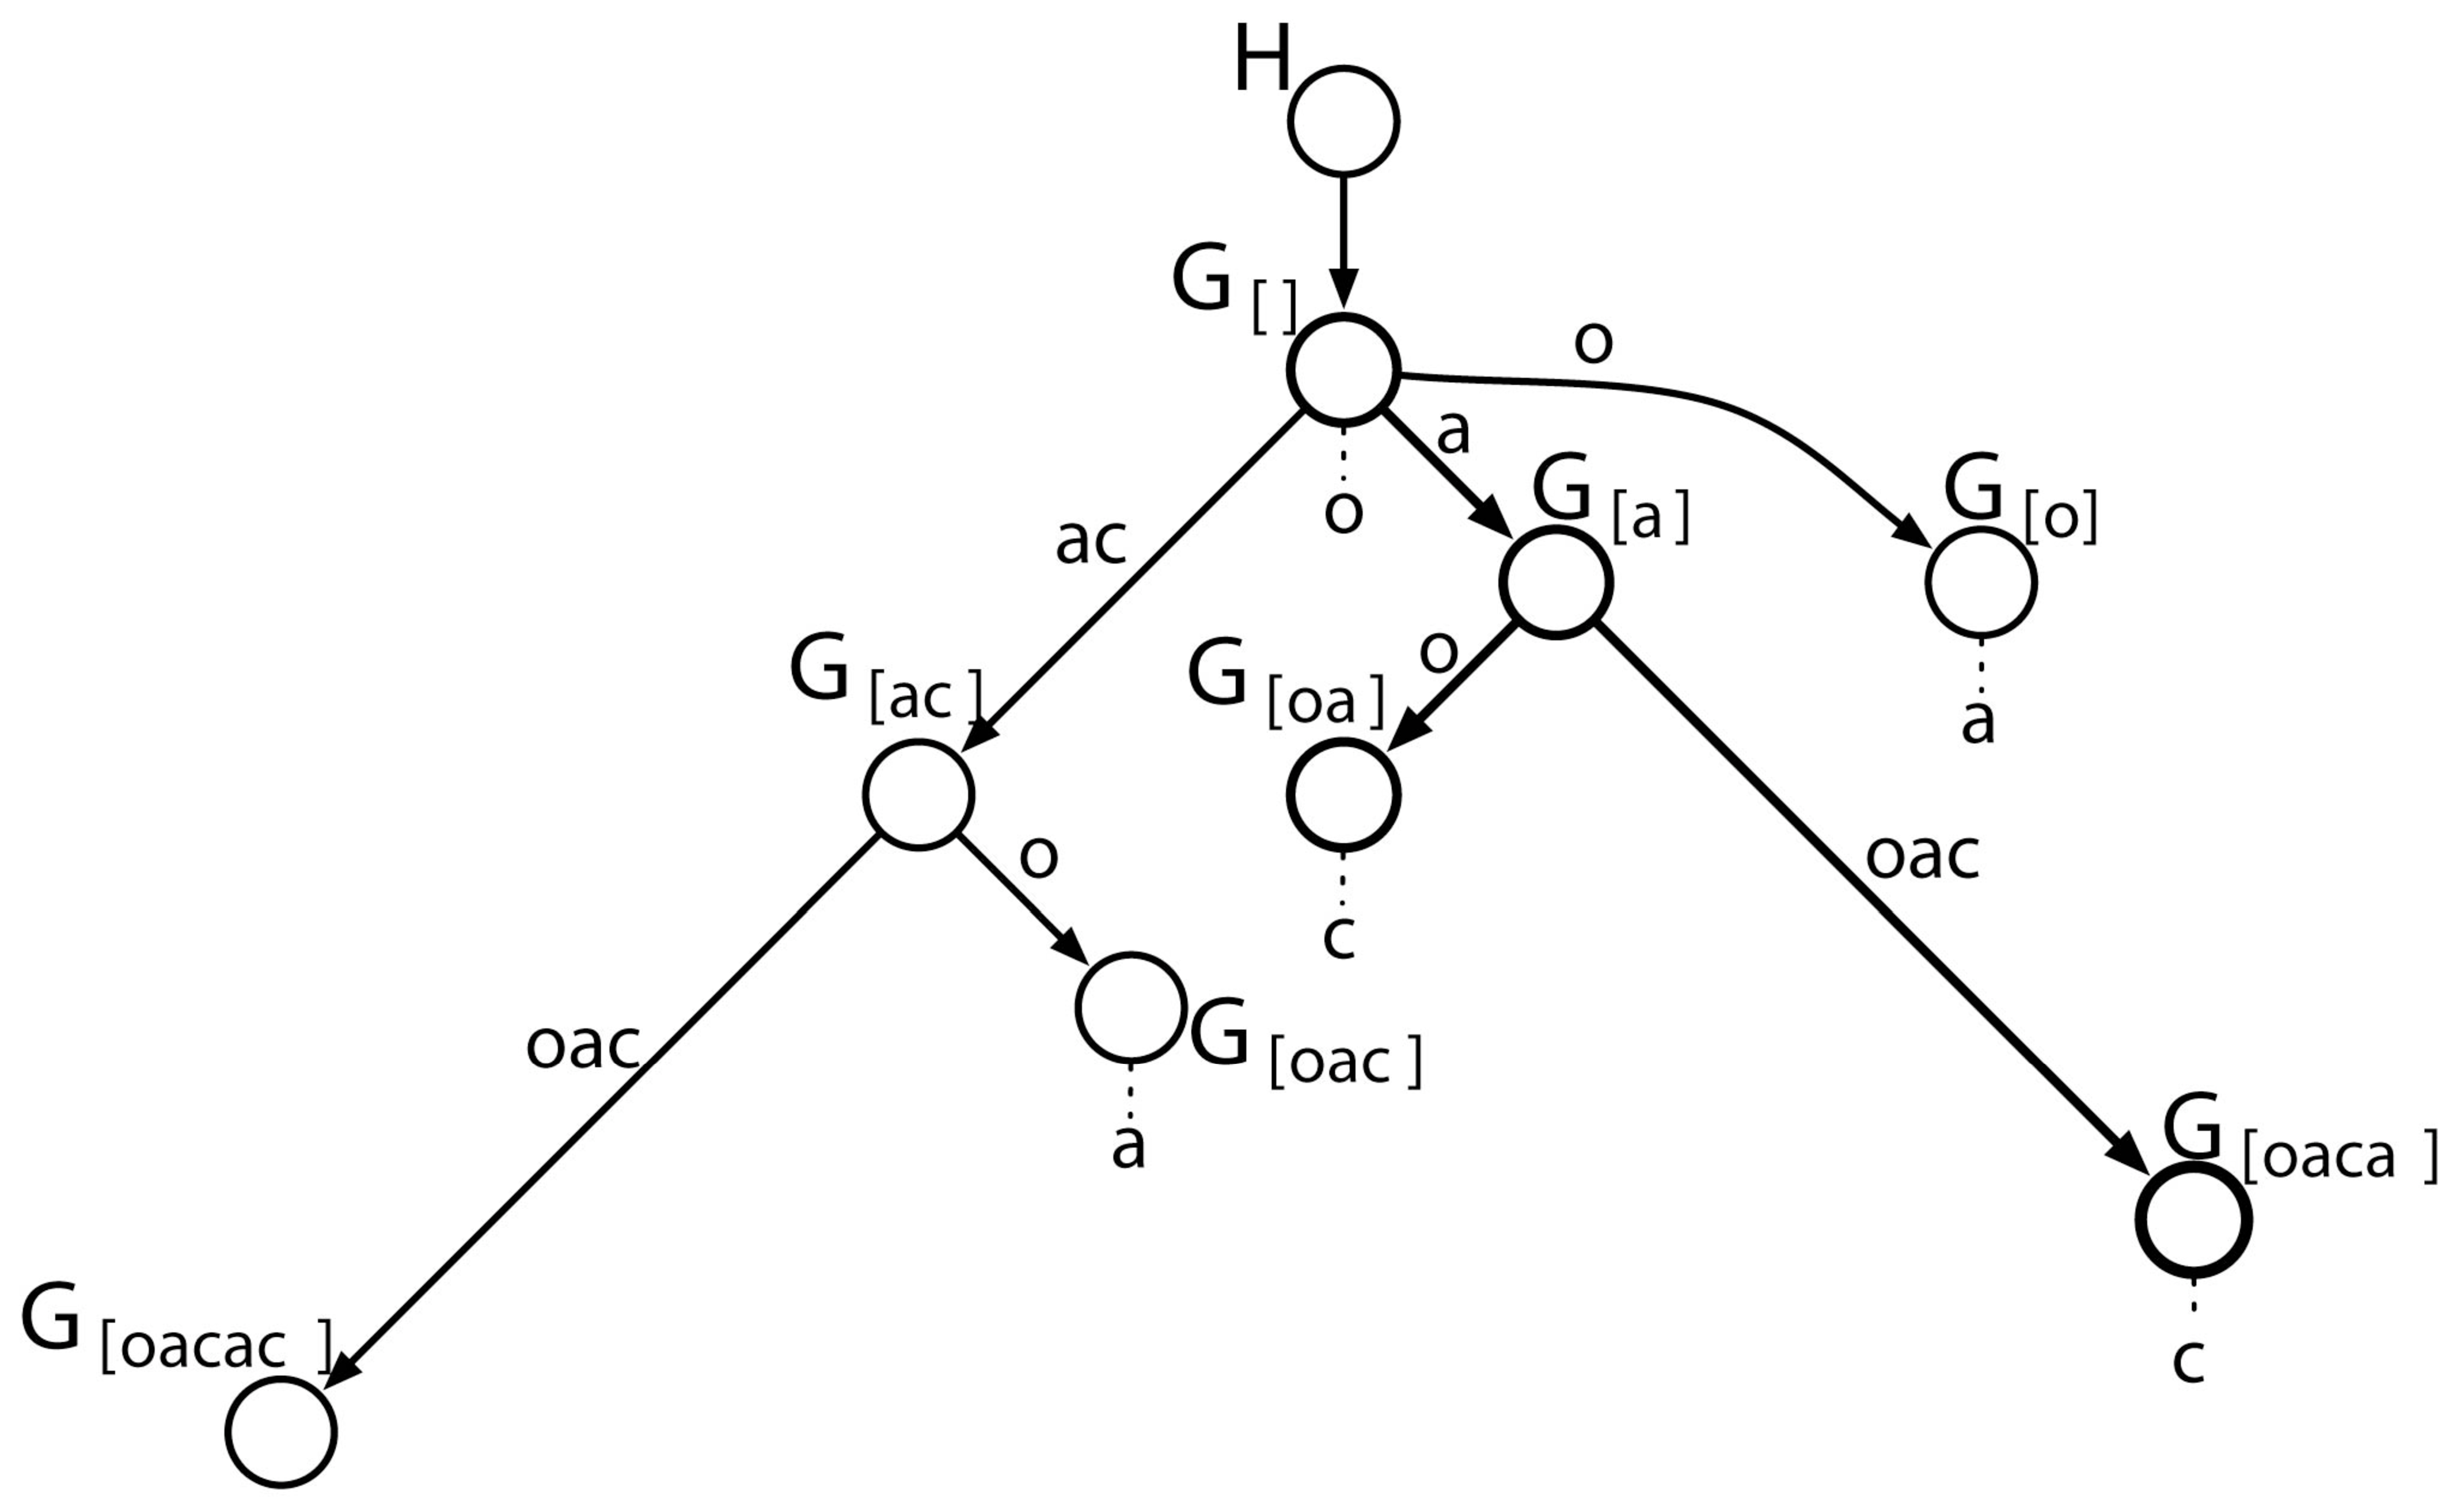
\includegraphics[height = 6cm, transparent]{figs/prefix_tree_not_coloured.pdf}
%		\end{center}
%	\end{figure}
%\end{frame}
%
%\begin{frame}[t]{Full Corpus Compression}
%
%	   	\begin{figure}[t]
%		\begin{center}
%			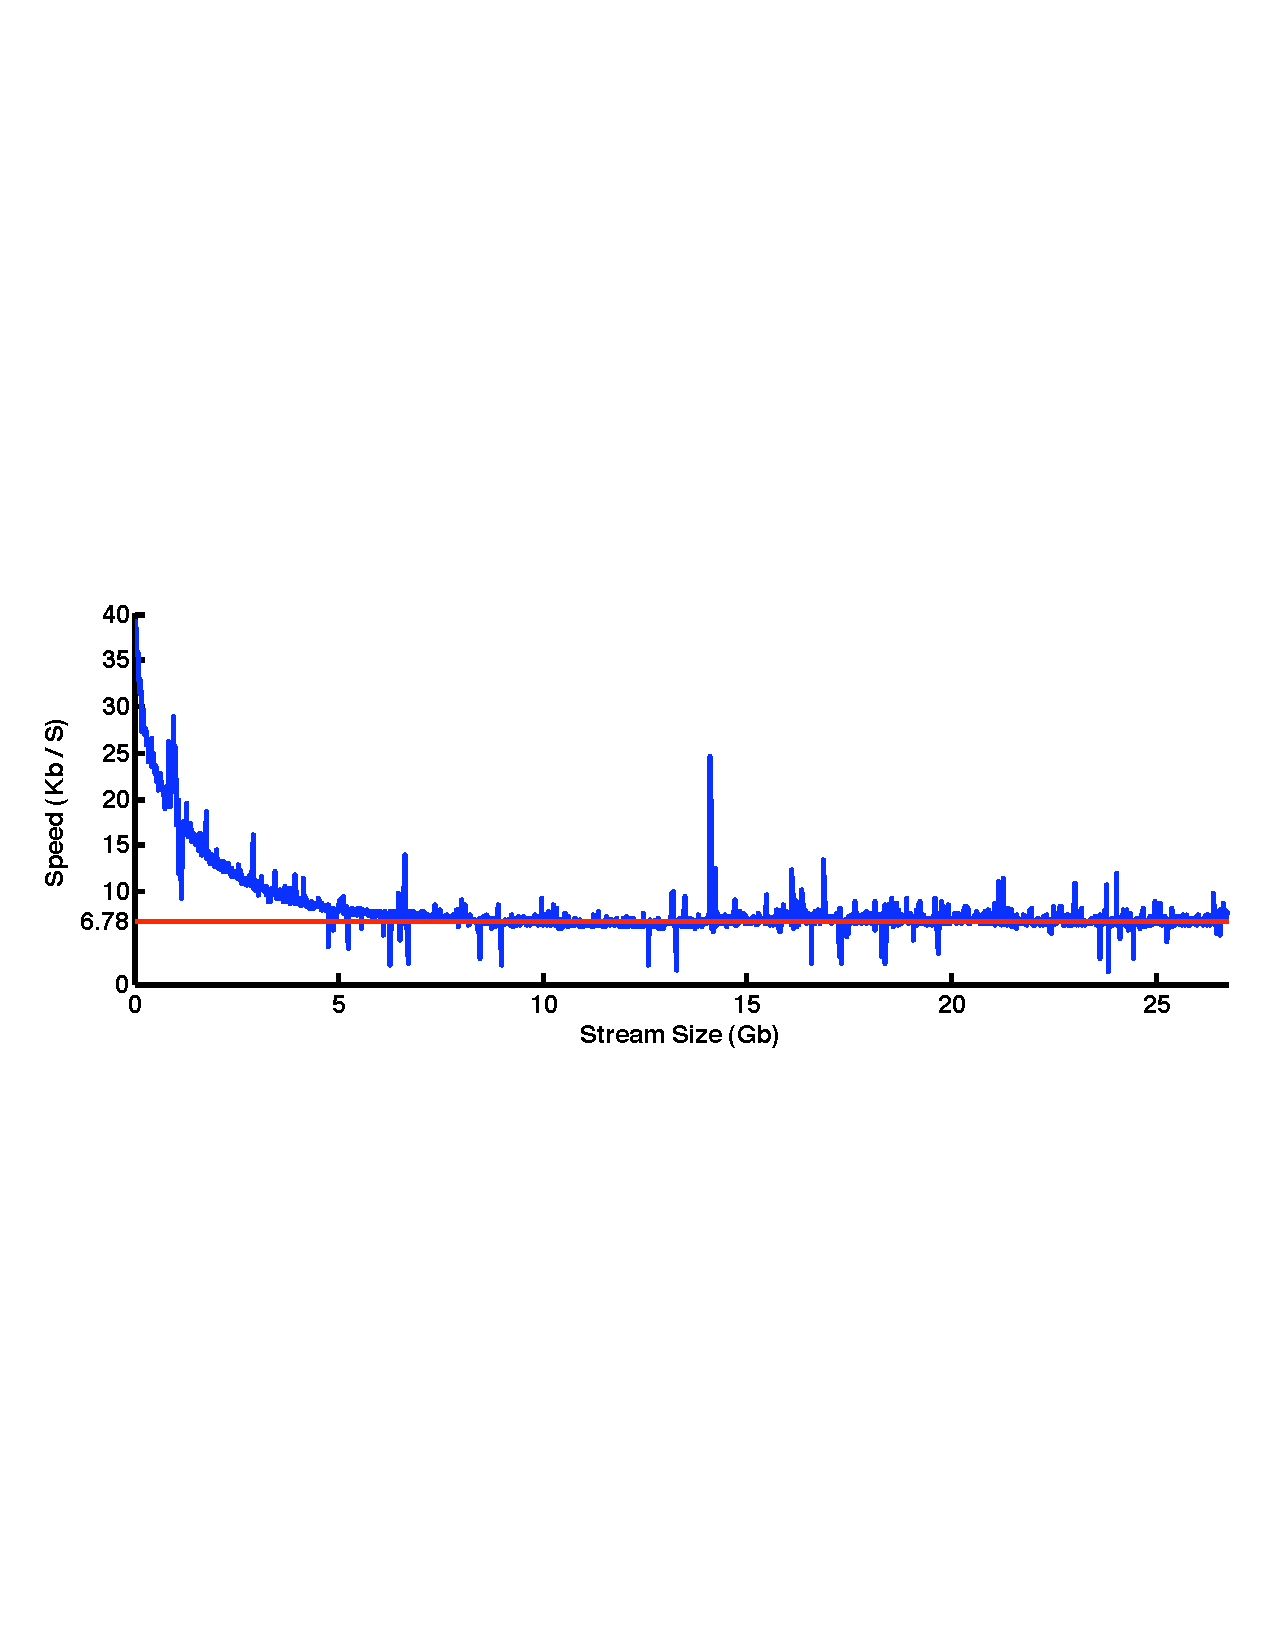
\includegraphics[width = 11cm]{figs/constant_speed_asymptote_small.pdf}
%		\end{center}
%	\end{figure}
%
%First streaming SM with computational asymptotics required for streaming compression.  Compressed 26.8Gb Wikipedia corpus to 4Gb (vs. 7.9Gb for gzip and 3.8Gb for PAQ).
%
%\end{frame}


	\bibliographystyle{plainnat}
	\begin{frame}[t,allowframebreaks]{Bibliography}

\bibliography{../../papers/uber}
\end{frame}

\begin{frame}[t]{ IEDHMM vs. IHMM }
	\begin{figure}[t]
		\begin{center}
			\includegraphics[width = .45\textwidth, transparent]{figs/iHMM-comparison-3d}
			\includegraphics[width = .45\textwidth, transparent]{figs/iHMM-reverse-comparison-3d}
		\end{center}
	\end{figure}
	{ \tiny Left: data from Poisson duration distribution ISEDHMM, Right: data from IHMM fit with Poisson duration distribution ISEDHMM}
\end{frame}

\frame[t] {
\frametitle{Poisson Process  \citep{Kingman:1993}}

Poisson process can be defined by the requirement that the random variables defined as the counts of the number of ``events'' inside each of a number of non-overlapping finite sub-regions of some space should each have a Poisson distribution and should be independent of each other.
\begin{figure}[t]
		\begin{center}
			\includegraphics[height = 4cm, transparent]{figs/poisson_process}
		\end{center}
	\end{figure}
\[N(A) \sim \mathsf{Poisson}(\mu(A)) \]
}

\frame[t] {
\frametitle{Gamma Process as Poisson Process \citep{Kingman:1993}}

Define a Poisson process over the product space $\Theta \otimes [0,\infty)$ with mean measure
\eqn \mu(\tilde\Theta, \tilde S) = \alpha(\tilde\Theta) \int_{\tilde S}\gamma^{-1}e^{-\gamma} \nonumber \enn
where $\tilde\Theta \in \Omega$ and $\tilde S \subset [0, \infty)$. A draw from this Poisson process yields a countably infinite set of pairs $\{ (\theta_{n}, \gamma_{n}) \}_{n \ge 1}$, which can be used to form an atomic random measure
\eqn G = \sum_{n \ge 1} \gamma_{n}\delta_{\theta_{n}}. \nonumber \enn

}

\frame[t] {
\frametitle{Gamma Process}


This discrete measure is draw from $G \sim \Gamma \textnormal P(\alpha)$ (from previous slide)

\eqn G = \sum_{n \ge 1} \gamma_{n}\delta_{\theta_{n}}. \nonumber \enn


A $\Gamma$P can be thought of as an unnormalized DP.

}

\frame[t] {
\frametitle{Dirichlet Processes}
%$G(\Theta)$ is finite with probability 1 \citep[pg.~93]{Kingman:1993}, so it can be normalized to yield a probability measure $D$. It is known that
 $D = G/G(\Theta)$ is a sample from a DP with base measure $\alpha$
\eqn D \sim \textnormal{DP}(\alpha). \nonumber \enn

A draw from a Dirichlet process is an infinite mixture of weighted, discrete atoms. \newline

For the ISEDHMM 

\begin{itemize}
\item each atom is a next state (there are a countably infinite number of such states)
\item each atoms' weight is the probability of transitioning to that state
\item there will be a countably infinite number of such transition distributions
\end{itemize}

%Note that Dirichlet processes are commonly written in terms of a concentration parameter $\alpha(\Theta)$ and the base {\em probability measure} $\alpha/\alpha(\Theta)$. We make use of the single parameter {\em measure} form.
}

\frame[t] {
\frametitle{Structured Transitions Via Dependent Dirichlet Processes}
\begin{itemize}
\item<1-3> One way to define a set of dependent DPs is to construct a base gamma process over an augmented space by taking the union of disjoint independent gamma processes, then define a series of restricted projections of that base process, which are themselves gamma processes. 

\item<2-3> The normalization of these dependent gamma processes form a set of dependent DPs.  

\item<3-3> We will use this procedure to construct a number of dependent DPs (one for each HMM state) which preclude certain transitions.  The precluded transitions, a form of dependence,  arise from particulars.
\end{itemize}

}


\begin{frame}[t]{ SN\GP~construction of IEDHMM transition distributions}
	\begin{figure}[t]
		\begin{center}
			\includegraphics[height = 6cm, transparent]{figs/ED-iHMM-hierarchical-model}
		\end{center}
	\end{figure}
	\citepalias{Huggins-2012-AISTATS}
\end{frame}



\frame[t] {
\frametitle{Spatial Normalized Gamma Processes \citep{Rao:2009}}
To review SN\GP s formally, let  $\mathbb V$ be an arbitrary auxiliary space.  In general, one can think of this as a covariate, time, or an index. 
% and, for the purposes of defining the IEDHMM, fix $\mathbb T$ and $\mathbb V$ to be the set of positive integers. For each $m \in \mathbb T$, define $V_{m}$ to be a subset of $\mathbb V$ which will serve to restrict the set of allowable transitions out of the state indexed by $m$. 
For $V \subset \mathbb V$, let  \begin{equation*} \alpha(\tilde\Theta, V) = c_{0}H_{\theta}(\tilde\Theta)H_{v}(V)\end{equation*}  be the base measure for a  gamma process $\mathcal G = \Gamma \textnormal P(\alpha)$ defined over the product space $\Theta \otimes \mathbb V$. Here $c_{0}$ is a concentration parameter and $H_{\theta}$ and $H_{v}$ are probability measures.  We will refer to  $\mathcal G$ as the ``base \GP''.  
}
%The states will thus be distributed in the auxiliary space according to $H_{v}$. We are not interested in where the latent states are in auxiliary space, however, so for each Dirichlet process $\mathbb V$ must be ``integrated out.''  For the DP associated with $m$, this marginalization is only performed over $V_{m}$, which has at the effect of tying DPs together since they will share point masses located in shared portions of the auxiliary space. In particular, 
\frame[t] {
\frametitle{Spatial Normalized Gamma Processes \citep{Rao:2009}}
\uncover<1->{Let $\mathbb T$ be an index set and define restricted projected measures $\alpha_{m}$ for all ${m \in \mathbb T}$ such that
\eqn \alpha_{m}(\tilde\Theta) = \alpha(\tilde\Theta, V_{m}) \label{eq:rpm} \nonumber \enn
where $V_{m}$ is a subset of $\mathbb V$ indexed by $m$. \newline}  

\uncover<2->{The SN\GP\,gets its name from thinking of $\mathbb V$ as a space and $V_m$ as a region of space indexed by $m$.
With $G \sim \mathcal G$ being a draw from the base gamma process, define the restricted projection $G_{m}$ by 
\eqn G_{m}(\tilde\Theta) =  G(\tilde\Theta, V_{m}). \label{eq:Gm} \nonumber\enn}%
\uncover<3->{Then $G_{m}(\tilde\Theta)$ is distributed according to a gamma process with base measure $\alpha_{m}$
\eqn  G_{m} \sim \Gamma \textnormal P(\alpha_{m}). \label{eq:rpgp} \nonumber\enn }

}

\frame[t] {
\frametitle{Spatial Normalized Gamma Processes \citep{Rao:2009}}
Normalizing $G_{m}$ yields a draw $D_{m} = G_{m}/G_{m}(\Theta)$ distributed according to a Dirichlet process with base measure $\alpha_{m}$
\eqn D_{m}  \sim \textnormal{DP}(\alpha_{m}). \label{eq:rpdp}\nonumber \enn
$D_{m}(\tilde \Theta)$ is not in general independent of $D_{m'}(\tilde \Theta)$ because they can share atoms from $G$.
}

\frame[t]{
\frametitle{IEDHMM \citepalias{Huggins-2012-AISTATS} (an example ISEDHMM)}

Recall the gamma process $\mathcal{G} = \Gamma \textnormal P(\alpha)$ with base measure \[\alpha(\tilde\Theta, V) = c_{0}H_{\theta}(\tilde\Theta)H_{v}(V).\]  Draws $G \sim \mathcal G$ are measures over the parameter and covariate product space  $\Theta \otimes \mathbb V$   %from the base $\Gamma$P for the SN$\Gamma$Ps defined in the previous section 
with the form
\eqn G  = \sum_{m=1}^{\infty} \gamma_{m} \delta_{(\theta_{m}, v_{m})} \nonumber \enn
where $(\theta_{m}, v_{m}) \sim H_{\theta}\times H_{v}$. \newline

In the IEDHMM $\theta_m = \{\lambda_m, \theta_m\}$ is the duration parameter and output distribution parameters for state $m$.  \newline

For pedagogical expediency let  $\mathbb T = \mathbb V = \{0,1,2,3,4,\ldots\}$ then $v_m \in \mathbb N$. 
%Without loss of generality (because $G$ identifies and orders a countable number of states), we  let $\mathbb T = \{1,2,3,\dots\}$, $\mathcal T = \{ 1, 2, \dots, M\}$, and $\mathcal V = \{v_{1}, v_{2}, \dots, v_{M}\}$. (i.e.~we can safely identify $M$ states for any dataset with fewer than $M$ observations.)

}

%\begin{frame}[t]{ISEDHMM: Geometric base distribution over states example}
%	\begin{figure}[t]
%		\begin{center}
%			\includegraphics[width=\textwidth, transparent]{figs/isedhmm_geom_base_gp}
%		\end{center}
%	\end{figure}
%\end{frame}

\begin{frame}[t]{IEDHMM: ``spatial'' regions for restrictions of base \GP}
\begin{alignat*}{2}
\mathsf R_{m} &= \{ v_{m} \} & \quad m  \in \mathcal T  \\
\mathsf R_{+} &= \mathbb V \setminus \mathcal V & \\
\mathcal R &= \{ \mathsf R_{m} : m \in \mathcal T \} \cup \{ \mathsf R_{+} \} & \\
\mathcal R_{m} &= \mathcal R \setminus \{ \mathsf R_{m} \} & \quad m \in \mathcal T 
\end{alignat*}
\end{frame}

\begin{frame}[t]{IEDHMM: Geometric base distribution over states example}
	\begin{figure}[t]
		\begin{center}
			\includegraphics[width=\textwidth, transparent]{figs/isedhmm_geom_base_gp}
		\end{center}
	\end{figure}
\end{frame}

\begin{frame}[t]{IEDHMM: SN\GP~restrictions}
\uncover<1->{From before, using the restricted projection $\alpha_{\mathsf R}(\tilde\Theta) = \alpha(\tilde\Theta, \mathsf R)$  setting $G_{\mathsf R}(\tilde\Theta) = G(\tilde\Theta, \mathsf R)$ and $D_{\mathsf R} = G_{\mathsf R} / G_{\mathsf R}(\Theta)$ we have 
\eqan
G_{\mathsf R} & \sim& \Gamma \textnormal P(\alpha_{\mathsf R}) \nonumber \\
D_{\mathsf R} & \sim& \textnormal{DP}(\alpha_{\mathsf R}). \nonumber
\enan}%
\uncover<2->{In the case of the IEDHMM,  the base measure corresponding to the point region $\mathsf R_{m} \in \mathcal R$ is 
\eqn \alpha_{\mathsf R_{m}}(\tilde\Theta) = c_{0}\delta_{\theta_{m}}(\tilde\Theta)H_{v}(\mathsf R_{m}), \nonumber \enn 
while for $\mathsf R_{+}$ it is 
\eqn \alpha_{\mathsf R_{+}}(\tilde\Theta) = c_{0}H_{\theta}(\tilde\Theta)H_{v}(\mathsf R_{+}). \nonumber \enn}
\end{frame}


\begin{frame}[t]{IEDHMM: From restricted \GP s to DPs}
	A {\em highly} dependent transition distribution for state $m$ is a DP draw $D_m$ 
\eqan
D_{m} &=& \frac{G_{m}}{G_{m}(\Theta)} = \frac{\sum_{\mathsf  R \in \mathcal R_{m}} G_{\mathsf  R}}{\sum_{\mathsf  R' \in \mathcal R_{m}} G_{\mathsf  R'}(\Theta)}  \nonumber \\
&=& \sum_{\mathsf  R \in \mathcal R_{m}} \frac{G_{\mathsf R}(\Theta)}{\sum_{\mathsf R' \in \mathcal R_{m}} G_{\mathsf R'}} \frac{G_{\mathsf R}}{G_{\mathsf R}(\Theta)}  \nonumber \\
&=& \sum_{\mathsf  R \in \mathcal R_{m}} \frac{G_{\mathsf R}(\Theta)}{\sum_{\mathsf R' \in \mathcal R_{m}} G_{\mathsf R'}} D_{\mathsf  R} \label{eq:DPmixture} \nonumber
\enan

\end{frame}


\frame[t] {
\frametitle{IEDHMM: Mixture of DP construction for transition distributions}
\eqan
D_{\mathsf  R_{m}} & \sim& \textnormal{DP}(\alpha_{\mathsf  R_{m}}) \nonumber  \\
D_{\mathsf R_{+}} & \sim & \textnormal{DP}(\alpha_{\mathsf R_{+}})  \nonumber\\
\gamma_{m} & \sim & \mathsf{Gamma}(c_{0}H_{v}(\mathsf R_{m}), 1) \nonumber \\
\gamma_{+}  & \sim & \mathsf{Gamma}(c_{0}H_{v}(\mathsf R_{+}), 1)  \nonumber \label{eq:gamma} \\
 \beta_{mk} & = & \frac{\mathbb I(m \ne k)\gamma_{k}}{\gamma_{+} + \sum_{k' \ne m}^{M} \gamma_{k'}}  \nonumber \\ 
\beta_{m+} & = &  \frac{\gamma_{+}}{\gamma_{+} + \sum_{k' \ne m}^{M} \gamma_{k'}}  \label{eq:beta} \nonumber \\
D_{m} & = &  \sum_{k \ne m}^{M} \beta_{mk} D_{\mathsf R_{k}} + \beta_{m+} D_{\mathsf R_{+}}.
\nonumber\enan
}

\frame[t] {
\frametitle{IEDHMM: Relaxing the dependence hierarchically}
These dependent DPs are the base dist.'s for conditional state transition distributions % from which the state transition counts $\bsym C = \{C_{mk}\}$ (with $C_{m+} = 0$) are drawn.  
    $\tilde D_{m}~\sim~\textnormal{DP}(c_{1}D_{m})$. With  $\bsym\beta_{m} = (\beta_{m1}, \dots, \beta_{mM}, \beta_{m+})$ 
\begin{align}
 \bsym\pi_{m} &\sim \mathsf{Dirichlet}(c_{1}\bsym\beta_{m}),   \label{eq:pi} \nonumber \\
 \tilde D_{m} &= \sum_{k=1}^{M} \pi_{mk}  \delta_{\theta_{m}} + \pi_{m+} D_{R_{+}}  \nonumber
\end{align}
where $c_{1}$ is a concentration parameter and $\bsym\pi_{m} = (\pi_{m1}, \dots, \pi_{mM}, \pi_{m+})$. \newline

The conditional state transition probability row vector $\bsym\pi_{m}$ is {\em finite}, since probabilities of transitioning to new states have been merged into a single probability $\pi_{m+} = \sum_{k=M+1}^{\infty} \pi_{mk}$.   This ``bin'' is dynamically split and joined at inference time.
}



\end{document}
